\section{Summary Statistics}

We now provide several tables that summarize features of the experiment. For example, we include tables listing the numbers of fish and which tanks they belonged to. Tables were created in R using the `kableExtra' package \citep{kable}.

\begin{table}[H]
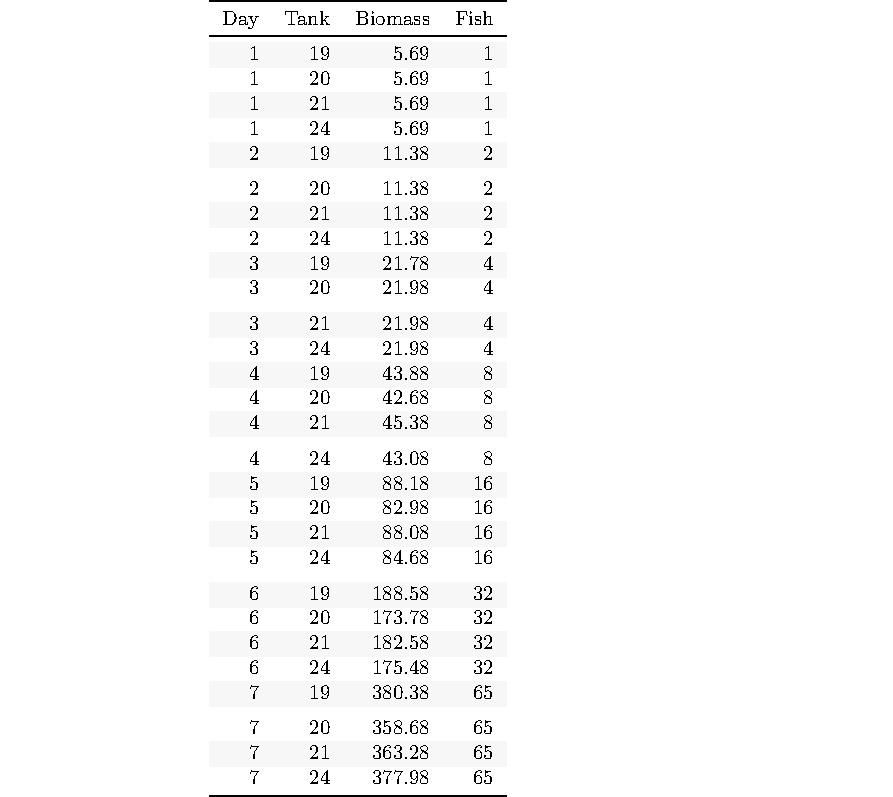
\includegraphics{Chapter3Images/kable1test.pdf}
\caption{Table summarizing biomass (g) per tank and day.}
\label{lab:kable1}
\end{table}

Table~\ref{lab:kable1} provides the weight and number of the fish in each tank. For every day for a week, the amount of fish in the tanks (and hence the biomass) was doubled (except on the seventh day, it was doubled plus one to make 65 fish)


\begin{table}[H]
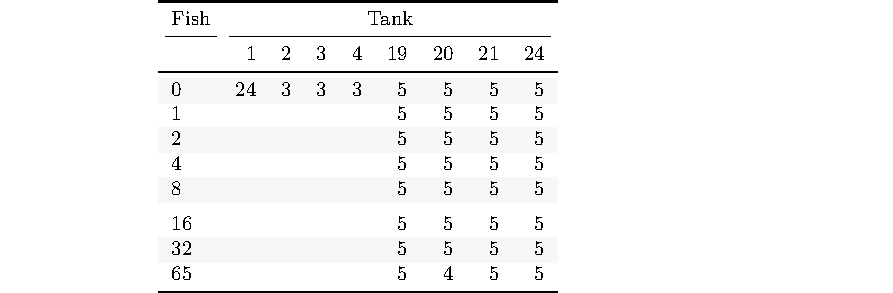
\includegraphics{Chapter3Images/kable2fixed2.pdf}
\caption{ Summary of the number of sample replicates for each corresponding number of fish and tank number.
}
\label{lab:kabel2}
\end{table}

Table~\ref{lab:kabel2} provides the number of sample replicates that were taken from each tank, and how many fish were present in that tank. Tanks 1, 2, 3, 4, 19, 20, 21 and 24 all had samples taken in which there were zero fish. However, for most levels of fish density, such as 16 fish or 32 fish, only tanks 19, 20, 21 and 24 were used. In general, five sample replicates were taken from each of the four main tanks for each level of fish density (except for tank 20, 65 fish).

\begin{table}[H]
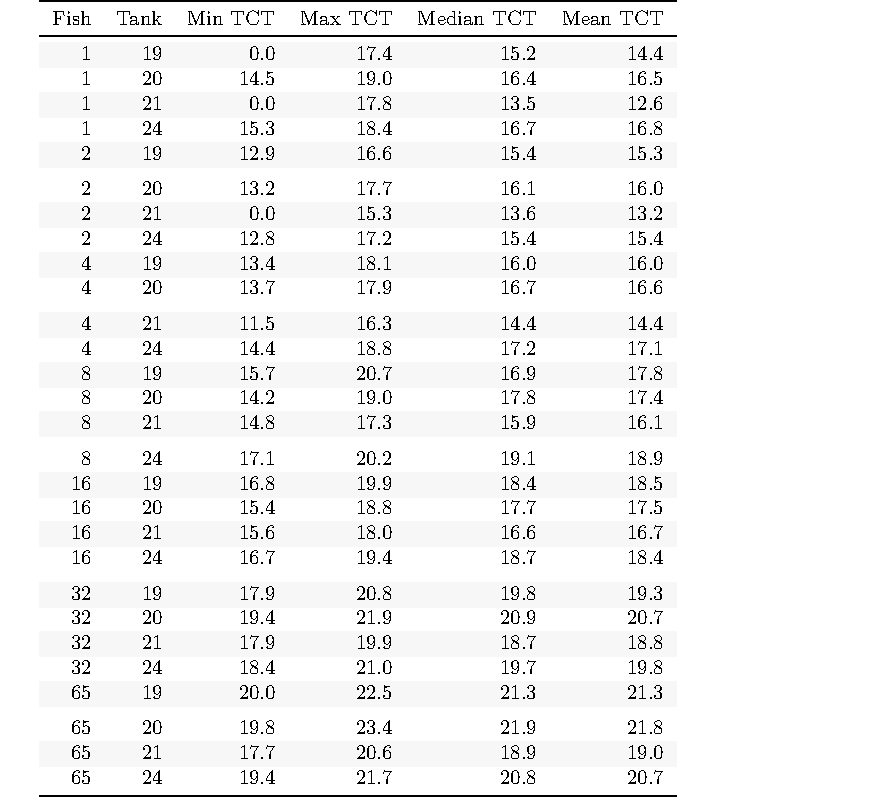
\includegraphics{Chapter3Images/kable3fixed2.pdf}
\caption{ Summary of the minimum, maximum and median TCT for each number of fish and tank.}
\label{lab:kabel3}
\end{table}

Table~\ref{lab:kabel3} provides several summary statistics for TCT values obtained. For each number of fish and tank, there were five sample replicates, and for each sample replicate there were eight technical replicates. Hence the maximum, minimum and median calculations use 5 x 8= 40 measurements each. Because one set of technical replicates was discarded from 65 fish, tank 20, only 32 measurements were used for that set of summary statistics.


\begin{table}[H]
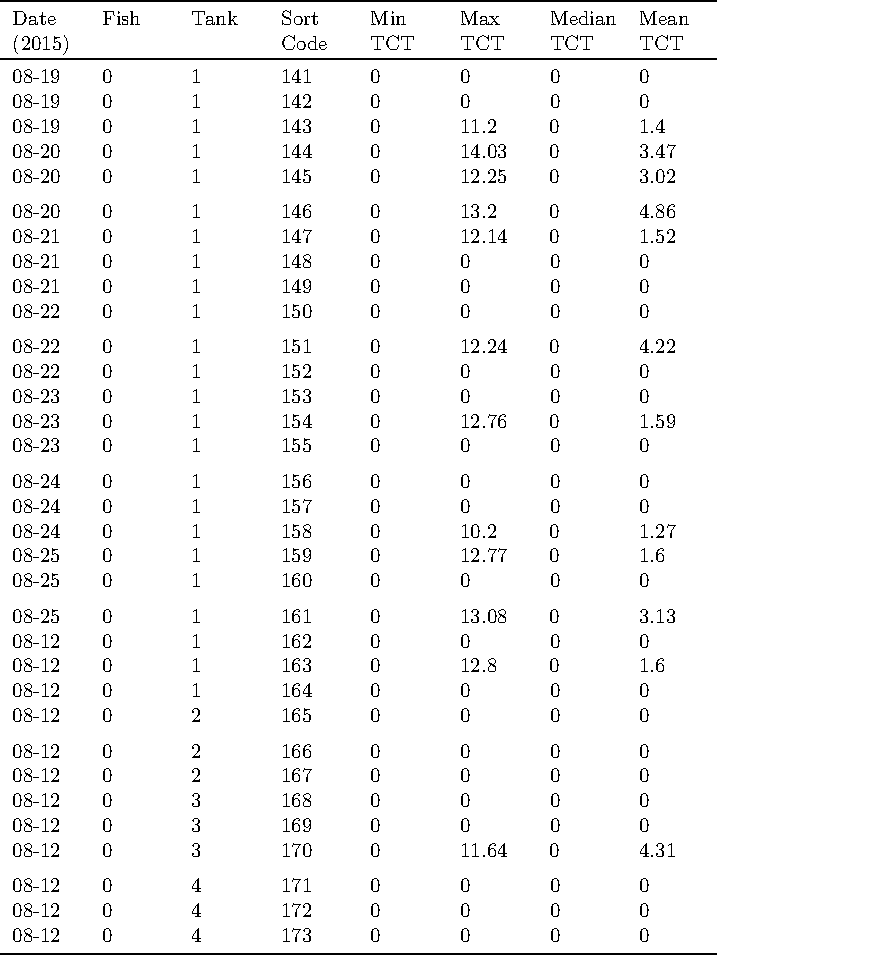
\includegraphics{Chapter3Images/kable4new.pdf}
\caption{  These samples correspond to the Pilot experiment. They were taken to give an insight on the TCT background signal at the hatchery. We include the date for which the sample was taken, the tank, the sort code, and the summary statistics.}
\label{lab:kabel4}
\end{table}

Table~\ref{lab:kabel4} summarizes the samples that were taken concurrently over the course of the seven days in which the density experiment took place. The sampling began on August 19, 2015 and continued until August 25, 2015. These samples correspond mostly to a smaller tank (tank 1) and were taken during the pilot experiments. Samples corresponding to sort codes 162-173 are also part of the pilot experiment but were taken earlier on a single day (August 12). 


Finally, we include a table that summarizes the negative controls for the four main tanks.

\begin{table}[H]
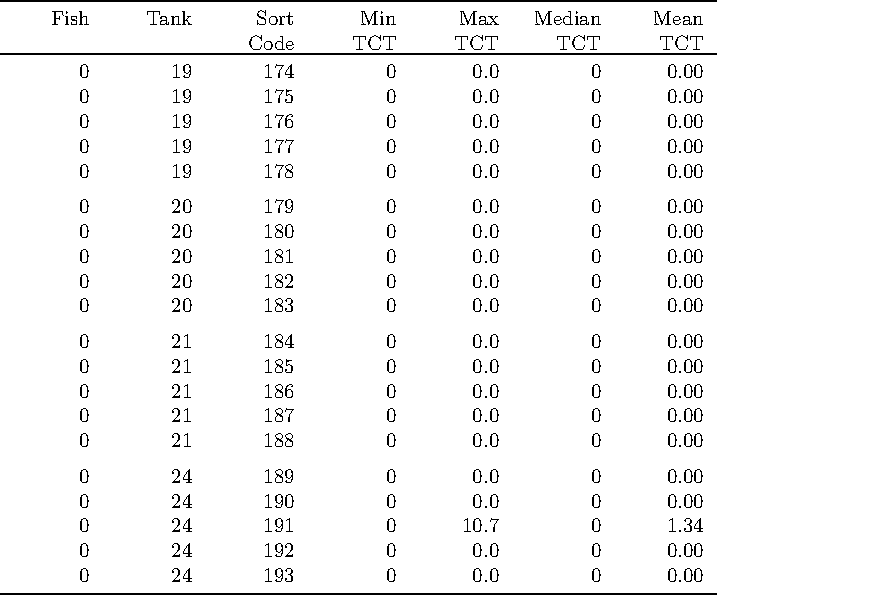
\includegraphics{Chapter3Images/kable5fixed2.pdf}
\caption{ Pre-fish, negative controls, taken over all of the tanks. The calculations are taken over the eight technical replicates. Notice we had a single TCT of 10.73 in tank 24, indicating an outlier. }
\label{lab:kabel5}
\end{table}



Table~\ref{lab:kabel5} summarizes the pre-fish negative controls. Samples were taken prior to the start of the experiment from the four main experiment tanks (tanks 19, 20, 21 and 24).